\begin{figure}[tbp]
\centering
\begin{subfigure}[b]{0.3\textwidth}
		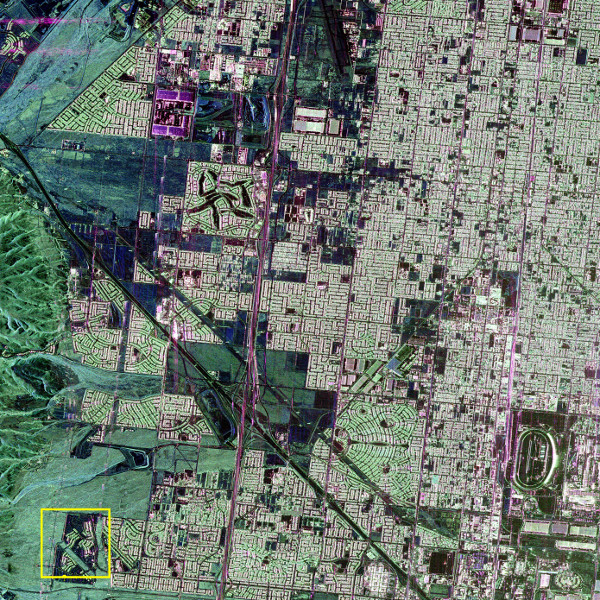
\includegraphics[width=\textwidth]{Figures/CD/2009}
		\caption{}
		\label{fig:2_a}
\end{subfigure}
\hspace{0.05pt}
\begin{subfigure}[b]{0.3\textwidth}
		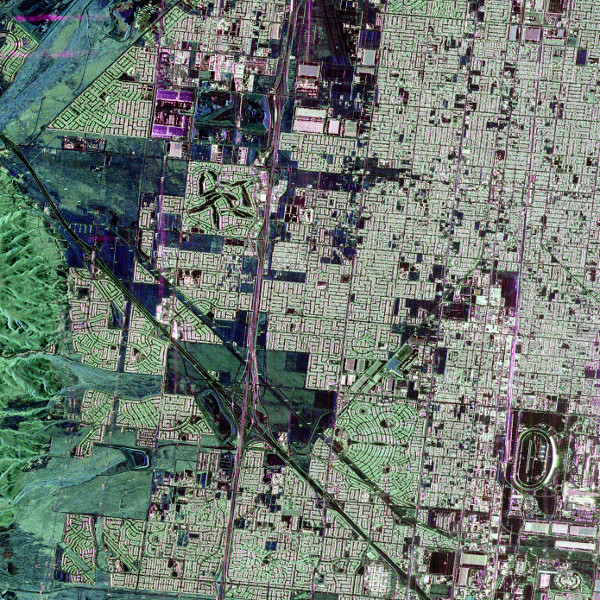
\includegraphics[width=\textwidth]{Figures/CD/2015.jpg}
		\caption{}
		\label{fig:2_b}
\end{subfigure}
\hspace{0.05pt}
\begin{subfigure}[b]{0.3\textwidth}
		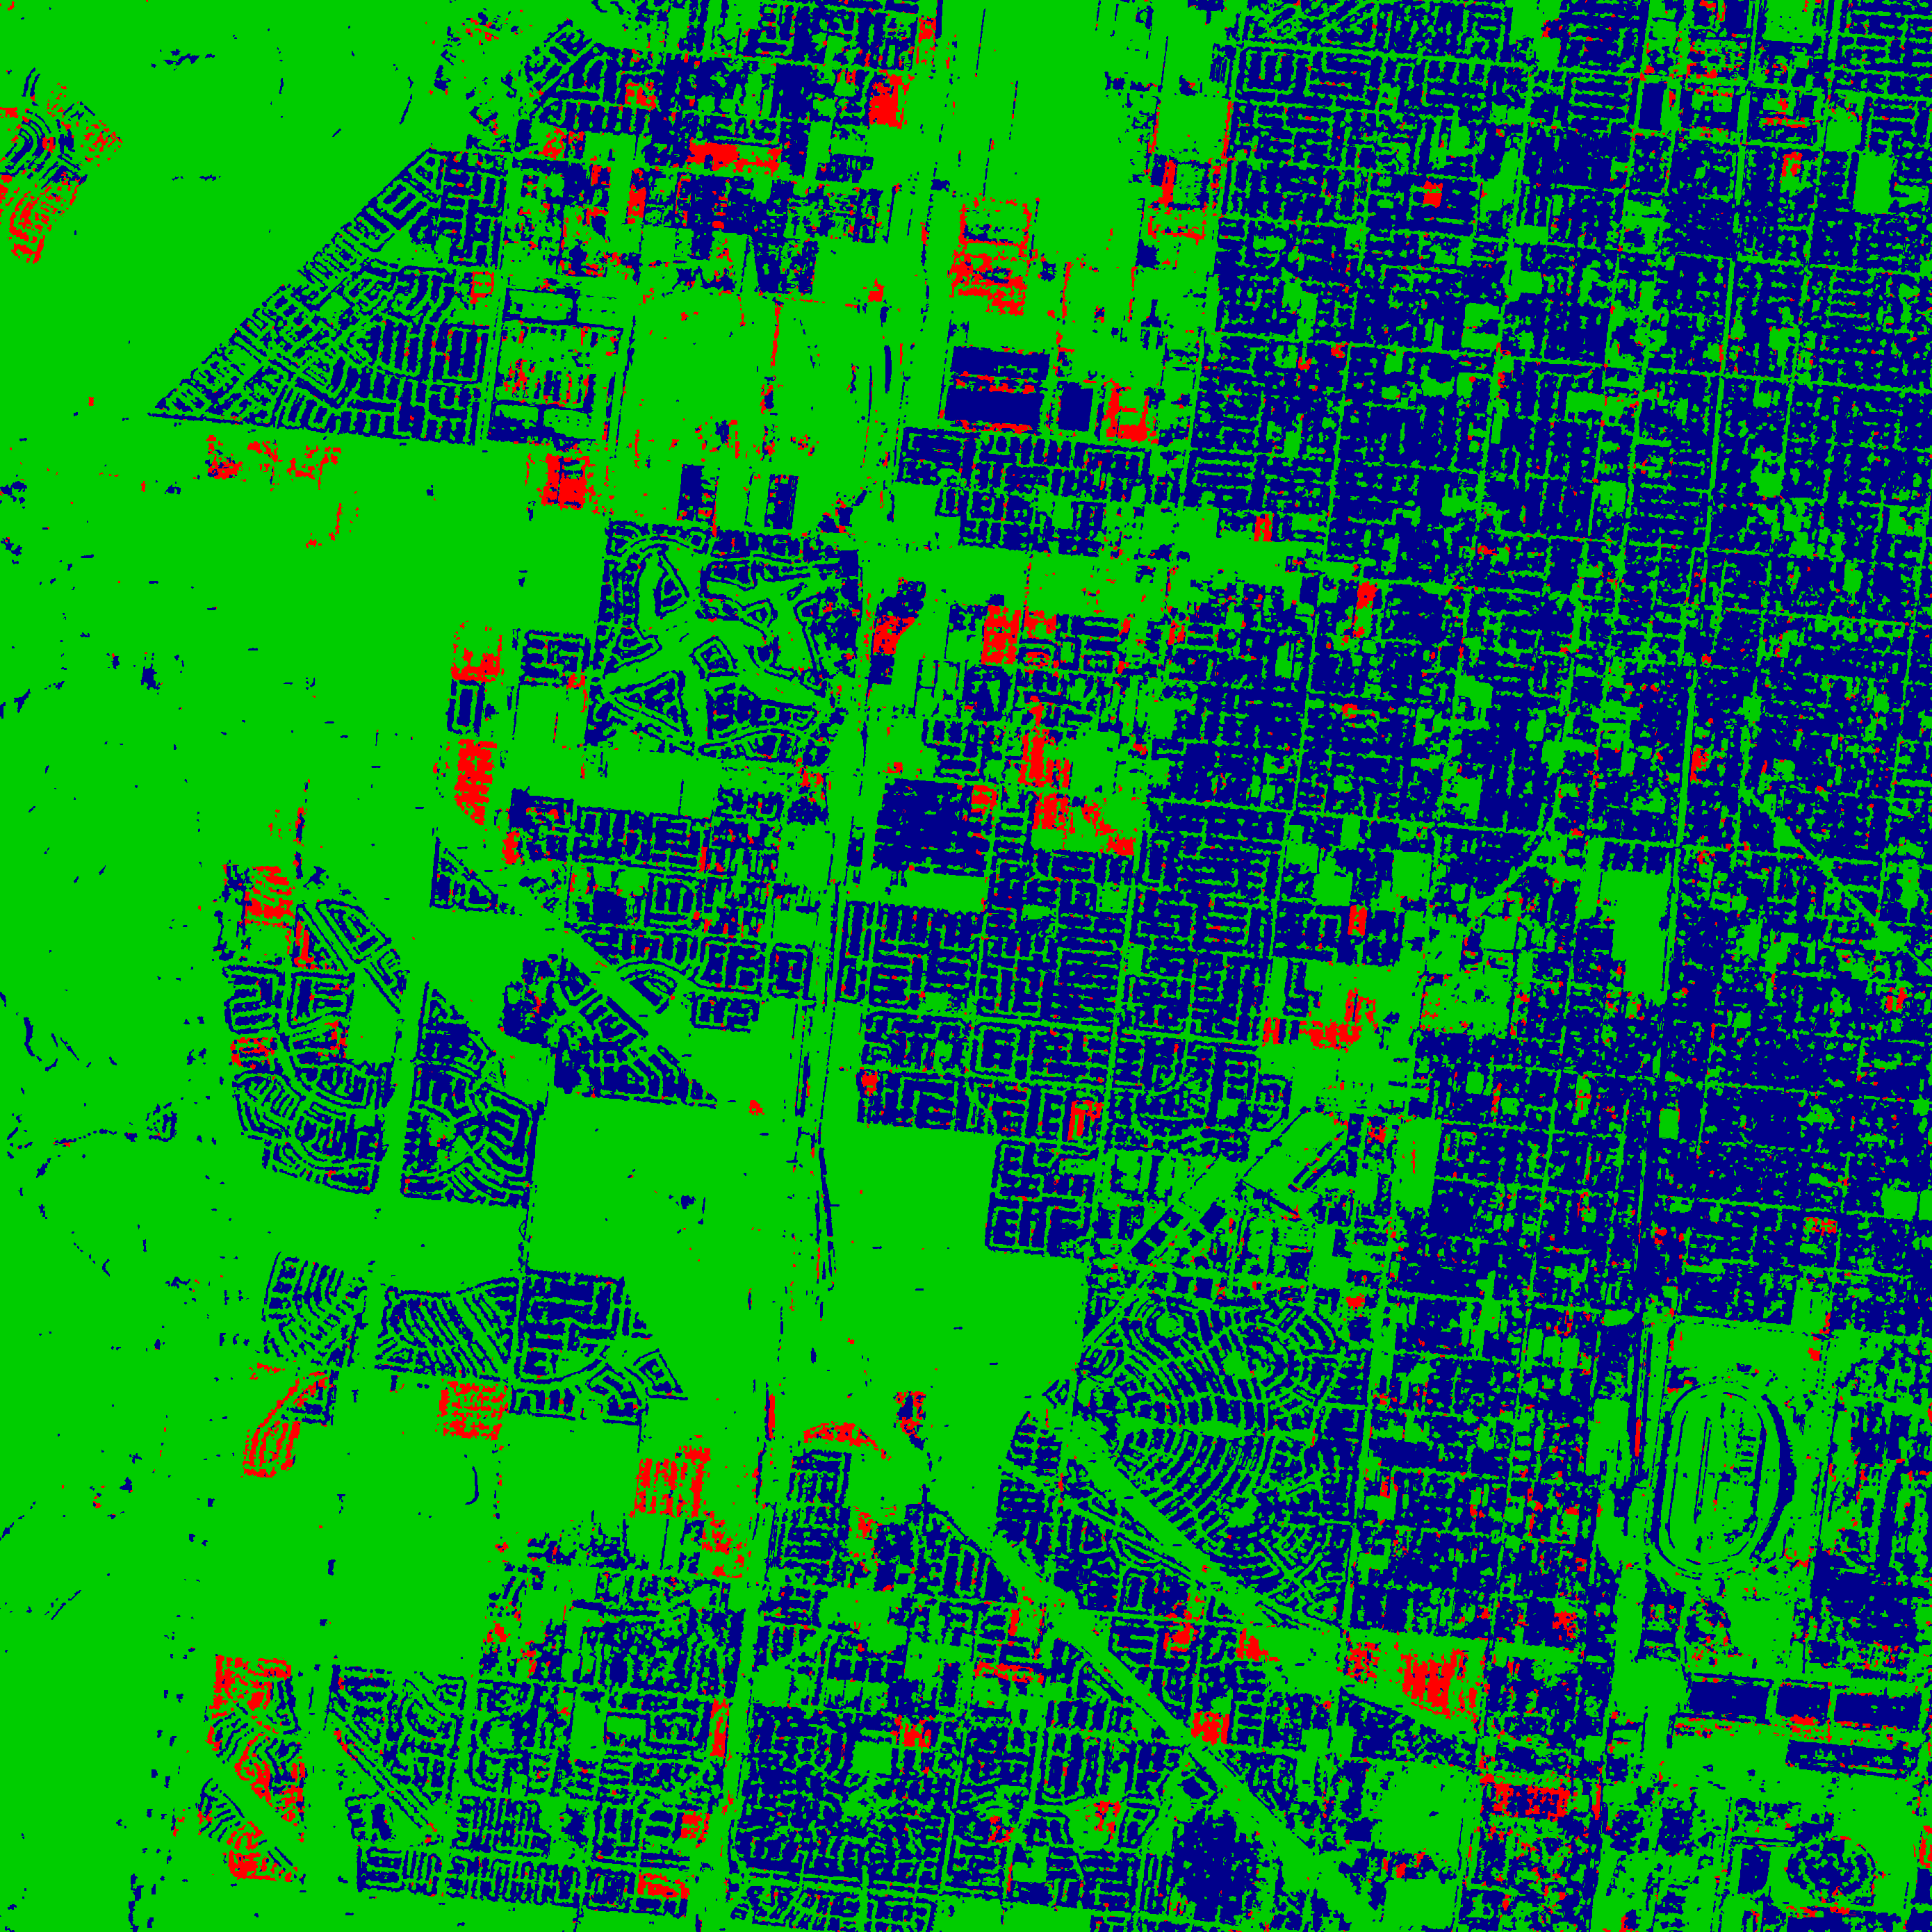
\includegraphics[width=\textwidth]{Figures/CD/result}
		\caption{}
		\label{fig:2_c}
\end{subfigure}

%\hspace{0.05pt}
\begin{subfigure}[b]{\textwidth}
\centering
		\vspace{0.2em}
		\begin{tabular}{ c l  c l  c l  }
	%	\hline
		 
\includegraphics[width=0.01\columnwidth]{Figures/CD/RED} & Urban Change (UC)  \hspace{1mm} &
		 
\includegraphics[width=0.01\columnwidth]{Figures/CD/GREEN} & Natural Unchanged (NU) \hspace{1mm} &
		 
\includegraphics[width=0.01\columnwidth]{Figures/CD/BLUE} & Urban Unchanged (UU) \hspace{1mm} \\
	%	\hline
		\end{tabular}
		%\vspace{20mm}
		%\caption{}
\end{subfigure}
\caption{The Pauli composite of (a) 2009, (b) 2015 image, and (c) the result of the classification. }
\label{fig:2}
\end{figure}

\begin{figure}[t]
\centering
\begin{subfigure}[b]{0.2\columnwidth}
		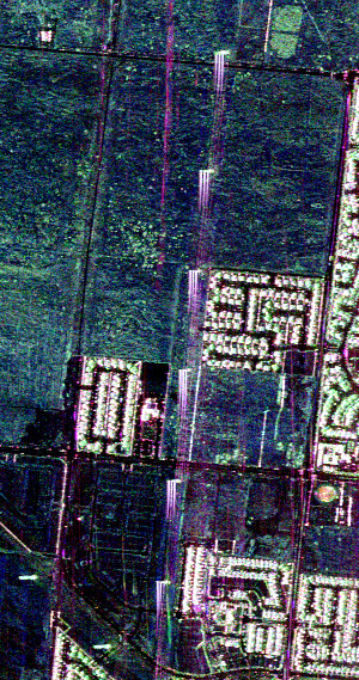
\includegraphics[width=\textwidth]{Figures/CD/A2_2009}
		\caption{}
		\label{fig:3_a}
\end{subfigure}
\hspace{0.01pt}
\begin{subfigure}[b]{0.2\columnwidth}
		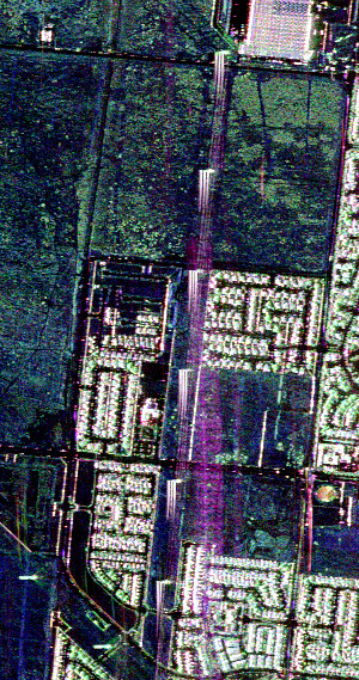
\includegraphics[width=\textwidth]{Figures/CD/A2_2015}
		\caption{}
		\label{fig:3_b}
\end{subfigure}
\hspace{0.01pt}
\begin{subfigure}[b]{0.2\columnwidth}
		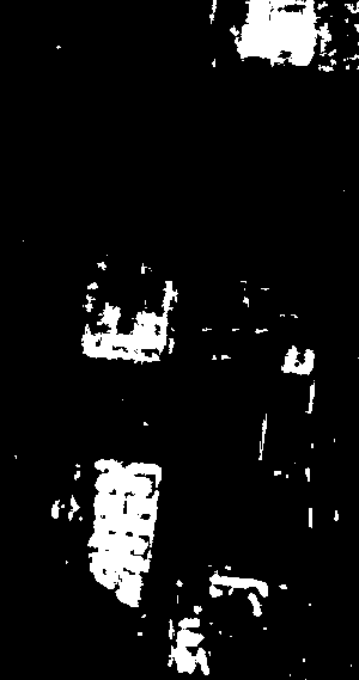
\includegraphics[width=\textwidth]{Figures/CD/REF_A2}
		\caption{}
		\label{fig:3_c}
\end{subfigure}
\hspace{0.01pt}
\begin{subfigure}[b]{0.2\columnwidth}
		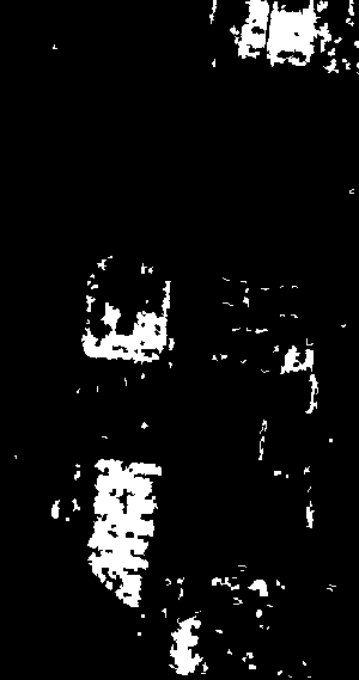
\includegraphics[width=\textwidth]{Figures/CD/OP_1_A2}
		\caption{}
		\label{fig:3_c}
\end{subfigure}

\begin{subfigure}[b]{\columnwidth}
\centering
		\vspace{0.2em}
		\begin{tabular}{c l  c l  }
		 
\includegraphics[width=0.02\columnwidth]{Figures/CD/BLK} & No Change   &
		 
\includegraphics[width=0.02\columnwidth]{Figures/CD/WHT} & Change
		\end{tabular}
\end{subfigure}
\caption{The Pauli composite of detail (a) 2009, (b) 2015 image, and the (c) reference change map, and (d) output change map.}
\label{fig:3}
\end{figure}

\subsection{Dataset and Study Area}
\label{sec:exp}
A pair of co-registered L-band ($\lambda = 0.23m$) UAVSAR images acquired over Los Angeles, California in 23-04-2009 and 11-05-2015 respectively  with a resolution of $0.4m$ in azimuth and $1.66m$ in range are used in this study. The dataset is multi-looked $2\times8$ times to form an effective pixel-size of $3.2m$.  The study-area is a dense urban area with changes occurring primarily due to the effects of urbanization. 

The objective of the proposed methodology is to  characterize the construction and destruction of urban areas, while simultaneously classifying unchanged urban and natural areas in the rest of the scene.
The major changes, i.e. `Changed Urban' class observed include the construction of suburban neighborhoods, industrial structures and public infrastructure like rail-yards and airports.  Natural areas of vegetation  comprise of the `Natural Unchanged' class. The urban infrastructure like houses, buildings, roads etc. that did not change is the 'Urban Unchanged' class.
%Thus the classes "Changed Urban" This represents both the changed urban areas and a land-cover classification of the unchanged areas: simultaneously generating an urban change and extent map.

%\section{Experimental Results and Discussion}
\subsection{Experimental Set-Up}
\label{sec:result}
The images are pre-processed and stacked to form the 20 dimensional input vector $x$.  The AE is a sparse 7-layer network comprised of 512, 256, 128 nodes in the encoder, 8 in the representational layer and 128, 256, 512 in the decoder with ReLU nodes. The auto-encoder is trained in an unsupervised manner with learning rate $\alpha=1e-5$ at initialization and is dropped by a step factor of $\Gamma=0.1$ every $100,000$ iterations.  After training,  $z$ is extracted from the representational layer and a PCA is applied pixel wise. It is seen that $k=3$ principal components contain most of the useful information.
% activation function used is ReLU. The learning rate $\alpha=1e-5$ at initialization and is dropped by a step factor of $\Gamma=0.1$ every $100,000$ iterations.
In a realistic scenario, reference information about the scene would only be available in a small portion of the area. Hence training samples are drawn from the part of the scene bounded by the yellow square in Figure~\ref{fig:2_a}. For each class $20$ pixels are labeled based on prior knowledge of the region and optical imagery. A total of $l=60$ training samples are  used, and $l<<N=9e6$ making the problem weakly supervised. A label aggregation step is performed by the ellipsoidal fitting technique described above. Reservoir sampling is performed to select $L=300$ labeled pixels per class from the points bounded by each ellipsoid. These aggregated labels are used to train a 3-layer MLP network with sigmoid activation function in a supervised manner. The final classification output   is shown in Figure~\ref{fig:2} along with the Pauli composition of the image pair. %The output simultaneously maps areas of changed urban ares, unchanged built-up and  natural land-cover. This is an improvement over outputs from  traditional ratio based methods that are unable to leverage the polarimetric information. 

\subsection{Results and Discussion}

\begin{table}[btp]
	\centering
	\caption{Confusion Matrix}
	\label{tab:conf}
	\begin{tabular}{cccc|c}
		&  UC (\%)  & NU (\%) & UU (\%) & Total \\ \hline
		UC (\%) & 90.28 & 0.34 &  0.00 & 26.11 \\
		NU (\%) & 2.24 & 88.54 & 1.10  & 35.91\\
		UU (\%) & 7.47 & 11.12 & 98.90 & 37.97\\ \hline
		OA   & 92.34\% &  $\kappa$   & 0.88 & \\ 
	\end{tabular}
	
\end{table}
\begin{table}[btp]
	\centering
	\caption{Change Detection Metrics}
	\label{tab:cd}
	\begin{tabular}{c c c c c c}
		PFP(\%)  & PFN(\%) & FA(\%) & DR(\%) & $\kappa$ \\ \hline
		0.89 & 1.75 & 2.64 & 82.3 & 0.83 \\
	\end{tabular}
\end{table}

Qualitatively, the  output corresponds well with the changed areas observed in the Pauli composition image pair and has low misclassification. Quantitatively, 
the confusion matrix is computed and presented in Table~\ref{tab:conf}.  The overall accuracy $OA = 92.34\%$ with $\kappa = 0.88$. The urban change (UC) areas are most commonly confused with the urban unchanged (UU) ones. This corresponds to areas where the learned representation was not sufficient to discriminate the two.
Another source of confusion is between natural unchanged (NU) and UU classes. The presence of vegetation intermixed with buildings in the UU areas makes it more difficult to discern it from the NU class leading to misclassification.
%The Pauli composition of the two images are shown in Figure~\ref{fig:3} with the 

To evaluate the CD capabilities the two unchanged classes, i.e. UU and NU are grouped together as a single unchanged class, with the UC representing the change as shown in Figure~\ref{fig:3}. Performance is evaluated in terms of false positive rate (PFP), false negative rate (PFN), false alarm rate (FA(\%)), detection rate (DR(\%)) and kappa (Table~\ref{tab:cd}). The method has a low FA rate of $FA=2.64\%$. This is due to design of the AE loss function and the radial thinning performed in the label aggregation step. The $DR=82.3\%$ can be improved at the cost of a higher $FA$, by eliminating the radial thinning step during label aggregation. The $\kappa=0.83$ indicates that there is very good agreement between the reference and output maps. This is confirmed qualitatively by visual inspection of the output image. 







%[[156301   1001]
% [  2844  10854]]
%[[ 0.99363644  0.00636356]
% [ 0.20762155  0.79237845]]
%Overall accuracy:
%97.7514619883
%Kappa:
%0.83744617901